\break
\section{Evaluation}

\subsection*{Overview}
The model was evaluated on a held-out test set of 1,732 breathing cycles. Each sample included a fused CLAP embedding of audio and patient metadata. The classification targets were \texttt{normal}, \texttt{crackles}, and \texttt{wheezes}.

\begin{figure}[htbp]
    \centering
    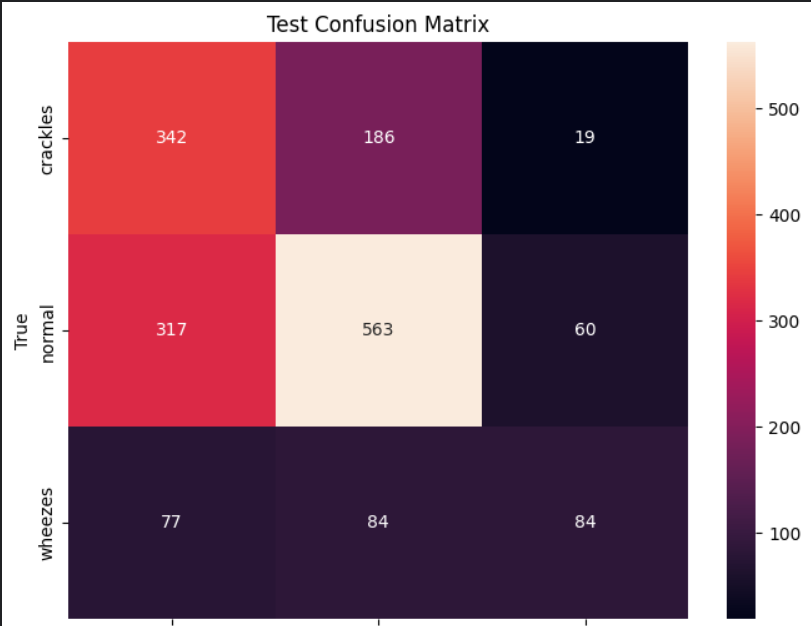
\includegraphics[width=0.7\linewidth]{Chapter4/pic.png}
    \caption{Test confusion matrix for respiratory sound classification.}
    \label{fig:confusion-matrix}
\end{figure}

\subsection{Performance Metrics}
\begin{itemize}
    \item \textbf{Accuracy:} 57.10\%
    \item \textbf{Macro F1-score:} 0.53
    \item \textbf{Weighted F1-score:} 0.57
    \item \textbf{Macro Precision:} 0.55
    \item \textbf{Macro Recall:} 0.52
\end{itemize}

\begin{table}[htbp]
\centering
\begin{tabular}{|l|c|c|c|c|}
\hline
\textbf{Class} & \textbf{Precision} & \textbf{Recall (Sensitivity)} & \textbf{F1-score} & \textbf{Support} \\
\hline
Crackles & 0.46 & 0.63 & 0.53 & 547 \\
Normal   & 0.68 & 0.60 & 0.64 & 940 \\
Wheezes  & 0.52 & 0.34 & 0.41 & 245 \\
\hline
\end{tabular}
\caption{Class-wise classification report.}
\end{table}

\subsection{Sensitivity and Specificity}
\begin{itemize}
    \item \textbf{Sensitivity (Recall):}
    \begin{itemize}
        \item Crackles: 0.625
        \item Normal: 0.599
        \item Wheezes: 0.343
        \item \textbf{Average:} 0.392
    \end{itemize}
    
    \item \textbf{Specificity:}
    \begin{itemize}
        \item Crackles: 0.668
        \item Normal: 0.659
        \item Wheezes: 0.947
        \item \textbf{Average:} 0.568
    \end{itemize}
\end{itemize}

\subsection{Observations}
\begin{itemize}
    \item The model performs best on the \texttt{normal} class, with an F1-score of 0.64.
    \item \texttt{Wheezes} are the hardest to classify (F1-score: 0.41), due to fewer examples and overlapping acoustic patterns with crackles.
    \item Specificity is highest for the \texttt{wheezes} class, indicating few false positives.
\end{itemize}

\subsection*{Summary}
The CLAP-based classifier shows promising overall accuracy and solid recall for crackles and normal sounds. Its lower sensitivity for wheezes suggests room for improvement through better balancing, augmentation, or fine-tuning the audio encoder. Still, the model maintains interpretability and scalability, aligning with the clinical goals of the system.
